%
% Sección de comparación de desempeño,
% presentación de TT 1.
%
% Proyecto Lovelace.
%

\subsection{Resultados}

\begin{frame}{Resultados}{Comparaciones de desempeño}

  \only<1>
  {
    {\small
      \begin{table}
        \begin{center}
          \begin{tabular}{c|c|c|c|c|}
            \cline{2-5}
            & \multicolumn{2}{c|}{100 oper.} & \multicolumn{2}{c|}{1K oper.} \\
            \cline{2-5}

            & Tok. & Detok. & Tok. & Detok. \\
            \hline
            \multicolumn{1}{|c|}{BPS} & 7.247 $m$s  & 6.990 $m$s  & 68.514 $m$s
              & 68.566 $m$s \\\cline{1-5}
            \multicolumn{1}{|c|}{FFX} & 5.627 $m$s  & 5.516 $m$s  & 49.738 $m$s
              & 49.550 $m$s \\\hline

            \multicolumn{1}{|c|}{TKR}   & 6.573 s  & 37.623 $m$s  & 70.116 s
              & 441.815$m$s \\\cline{1-5}
            \multicolumn{1}{|c|}{AHR}   & 6.053 s  & 58.814 $m$s  & 65.631 s
              & 420.729$m$s \\ \cline{1-5}
            \multicolumn{1}{|c|}{DRBG}  & 6.718 s  & 40.265 $m$s  & 71.082 s
              & 436.753$m$s \\\hline
          \end{tabular}

          \caption{Comparación de tiempos de tokenización.}
          \label{tabla:tiempos_tokenizacion}
        \end{center}
      \end{table}
    }
  }

  \only<2>
  {
    \begin{figure}[H]
      \begin{center}
        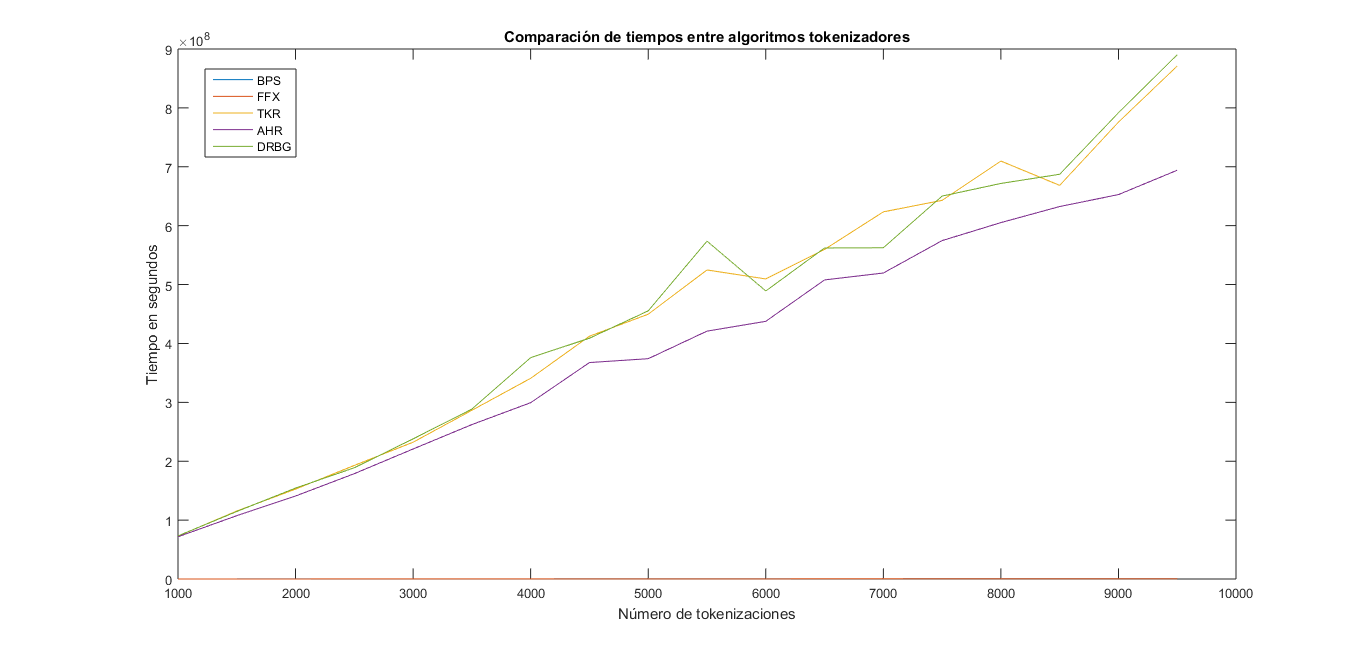
\includegraphics[width=1.0\linewidth]
          {../../../diagramas_comunes/desempenio/tok_todos.png}
        \caption{Tiempos de tokenización generales.}
      \end{center}
    \end{figure}
  }

  \only<3>
  {
    \begin{figure}[H]
      \begin{center}
        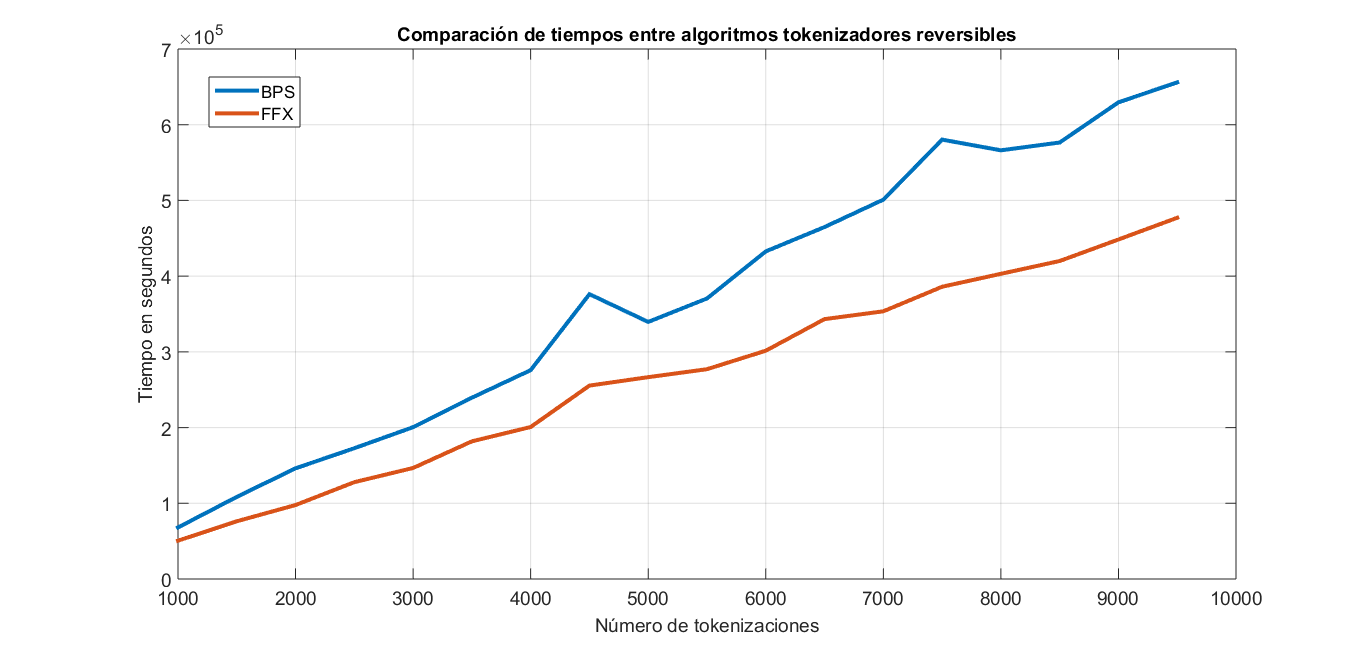
\includegraphics[width=1.0\linewidth]
          {../../../diagramas_comunes/desempenio/tok_rev.png}
        \caption{Tiempos de tokenización de reversibles.}
      \end{center}
    \end{figure}
  }

  \only<4>
  {
    \begin{figure}[H]
      \begin{center}
        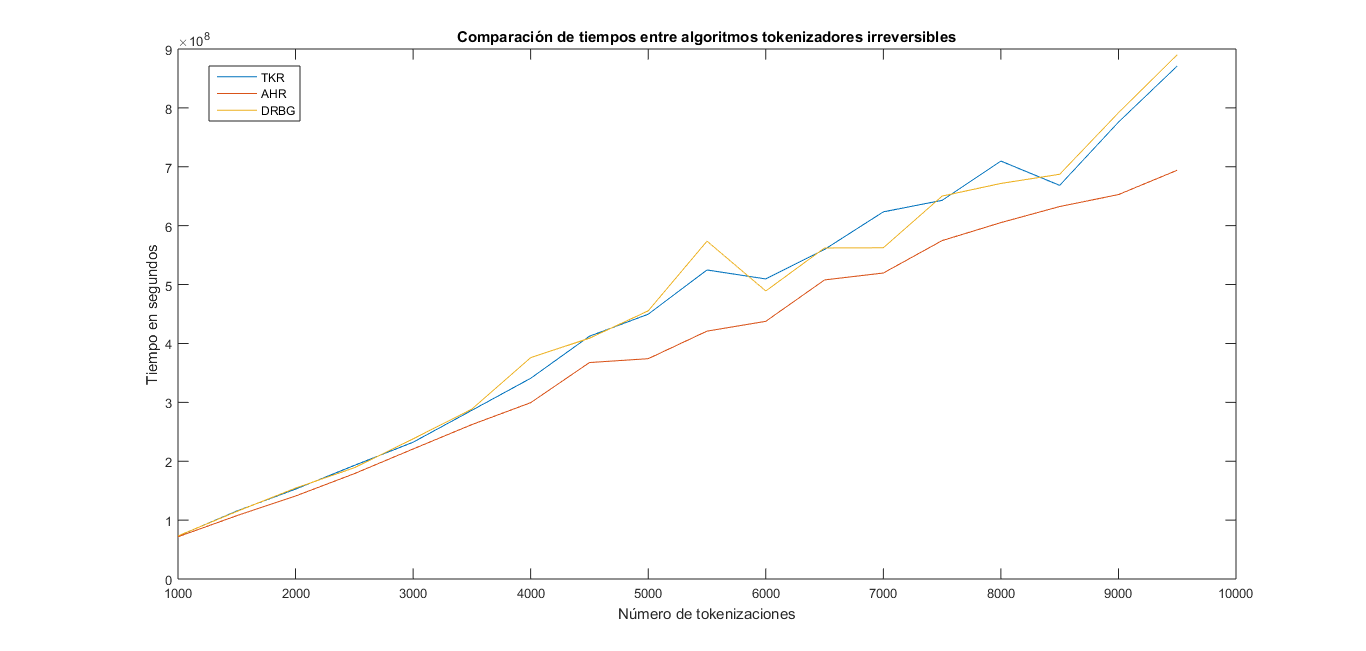
\includegraphics[width=1.0\linewidth]
          {../../../diagramas_comunes/desempenio/tok_irrev.png}
        \caption{Tiempos de tokenización de irreversibles.}
      \end{center}
    \end{figure}
  }

  \note
  {
    Los tiempos de los reversibles son mucho más cortos.

    Las gráficas muestran solo los procesos de tokenización: con la
    detokenización pasan cosas bastante similares.
  }

\end{frame}

\begin{frame}{Resultados}{Pruebas de aleatoriedad}

  En \cite{nist_pruebas} el NIST describe un conjunto de pruebas estadísticas
  que sirven para determinar la aleatoriedad de un generador pseudoaleatorio.
  Se trata de 15 pruebas generales (algunas de ellas con subpruebas) que es
  necesario ejecutar sobre los bits generados.

  Para cada instancia de los generadores implementados se ejecutó el conjunto
  de pruebas 20 veces, cada una con medio millón de bits (un total de veinte
  millones).

  \only<1>
  {
    Resultados para generador basado en función hash:
    \begin{itemize}
      \item 112 bits de seguridad: 14 de 15.
      \item 128 bits de seguridad: 15 de 15.
      \item 192 bits de seguridad: 14 de 15.
      \item 256 bits de seguridad: 15 de 15.
    \end{itemize}
  }

  \only<2>
  {
    Resultados para generador basado en cifrador por bloques:
    \begin{itemize}
      \item 112 bits de seguridad: 15 de 15.
      \item 128 bits de seguridad: 15 de 15.
      \item 192 bits de seguridad: 15 de 15.
      \item 256 bits de seguridad: 15 de 15.
    \end{itemize}
  }

  \note
  {
    Estrictamente hablando, el generador basado en una función hash no es
    totalmente aleatorio, dado que falló en un par de pruebas. Sin embargo,
    el número de veces que se ejecutó el conjunto de pruebas (veinte) es
    un número relativamente pequeño (en comparación con lo recomendado por
    el NIST); esto por los recursos de cómputo que las pruebas exigen. 
  }

\end{frame}
